%%%%%%%%%%%%%%%%%%%%%%%%%%%%%%%%%%%%%%%%%
% Journal Article
% LaTeX Template
% Version 1.3 (9/9/13)
%
% This template has been downloaded from:
% http://www.LaTeXTemplates.com
%
% Original author:
% Frits Wenneker (http://www.howtotex.com)
%
% License:
% CC BY-NC-SA 3.0 (http://creativecommons.org/licenses/by-nc-sa/3.0/)
%
%%%%%%%%%%%%%%%%%%%%%%%%%%%%%%%%%%%%%%%%%

%----------------------------------------------------------------------------------------
%	PACKAGES AND OTHER DOCUMENT CONFIGURATIONS
%----------------------------------------------------------------------------------------

\documentclass[twoside]{article}

\usepackage{lipsum} % Package to generate dummy text throughout this template

\usepackage[sc]{mathpazo} % Use the Palatino font
\usepackage[T1]{fontenc} % Use 8-bit encoding that has 256 glyphs
\linespread{1.05} % Line spacing - Palatino needs more space between lines
\usepackage{microtype} % Slightly tweak font spacing for aesthetics

\usepackage[hmarginratio=1:1,top=32mm,columnsep=20pt]{geometry} % Document margins
\usepackage{multicol} % Used for the two-column layout of the document
\usepackage[hang, small,labelfont=bf,up,textfont=it,up]{caption} % Custom captions under/above floats in tables or figures
\usepackage{booktabs} % Horizontal rules in tables
\usepackage{float} % Required for tables and figures in the multi-column environment - they need to be placed in specific locations with the [H] (e.g. \begin{table}[H])
%\usepackage{hyperref} % For hyperlinks in the PDF

\usepackage{lettrine} % The lettrine is the first enlarged letter at the beginning of the text
\usepackage{paralist} % Used for the compactitem environment which makes bullet points with less space between them
\usepackage{parskip} % turns off indentation and adds a little bit of (stretchable) space in between paragraphs

\usepackage{abstract} % Allows abstract customization
\renewcommand{\abstractnamefont}{\normalfont\bfseries} % Set the "Abstract" text to bold
\renewcommand{\abstracttextfont}{\normalfont\small\itshape} % Set the abstract itself to small italic text

\usepackage{titlesec} % Allows customization of titles
%\renewcommand\thesection{\Roman{section}} % Roman numerals for the sections
%\renewcommand\thesubsection{\Roman{subsection}} % Roman numerals for subsections
\titleformat{\section}[block]{\large\scshape\centering}{\thesection.}{1em}{} % Change the look of the section titles
\titleformat{\subsection}[block]{\large}{\thesubsection.}{1em}{} % Change the look of the section titles

\usepackage{fancyhdr} % Headers and footers
\pagestyle{fancy} % All pages have headers and footers
\fancyhead{} % Blank out the default header
\fancyfoot{} % Blank out the default footer
\fancyhead[C]{Autonomous Systems Engineering} % Custom header text
\fancyfoot[RO,LE]{\thepage} % Custom footer text

\usepackage{graphicx}
\usepackage{multicol}
\usepackage{tikz}
\usepackage{textcomp}
\usepackage{wrapfig}
\usepackage{floatflt}
\usetikzlibrary{shapes}
% Quellcode
\usepackage{listings}
\lstloadlanguages{C++,Python}
\definecolor{mygreen}{rgb}{0,0.6,0}
\definecolor{myblue}{rgb}{0,0,0.8}
\lstset{ %
	breaklines=true,
	basicstyle=\fontsize{10pt}{12pt}\ttfamily,
	commentstyle=\color{mygreen},
	keywordstyle=\color{myblue},
	rulecolor=\color{black},
	captionpos=b,
	language=Python,
	numbers=left,
	xleftmargin=2em,
	numberstyle=\tiny,
	framexleftmargin=1.8em,
	%numbersep=10pt,
	frame=L}
%----------------------------------------------------------------------------------------
%	TITLE SECTION
%----------------------------------------------------------------------------------------

\title{\vspace{-15mm}\fontsize{24pt}{10pt}\selectfont\textbf{Scenario and Evaluation Algorithms}} % Article title

\author{
\large
\textsc{Hendrik Oestreich, Andreas Gatting, Timo Michalski, Julian Daberkow}\\
\textsc{Julian Exner, <further Authors>}\\%\thanks{A thank you or further information}\\[2mm] % Your name
\normalsize University of Bielefeld \\ % Your institution
%\normalsize hoestreich@techfak.uni-bielefeld.com%\href{mailto:hoestreich@techfak.uni-bielefeld.com}{hoestreich@techfak.uni-bielefeld.com} % Your email address
%\vspace{-5mm}
}
\date{July 2015}

%----------------------------------------------------------------------------------------

\begin{document}

\maketitle % Insert title

\thispagestyle{fancy} % All pages have headers and footers


%----------------------------------------------------------------------------------------
%	ARTICLE CONTENTS
%----------------------------------------------------------------------------------------

%\begin{multicols}{2} % Two-column layout throughout the main article text

\section{Scenario}
\subsection{Teleworkbench}
The teleworkbench (TWB) is a laboratory for evaluation and tracking purposes of mutli-robot scenarios in the CITEC of the University of Bielefeld. An area of 6x6m is tracked by a camera array of 4 cameras mounted at the ceiling. The rest of the room is workspace and used for controlling the experiments in the testing area. 

\subsection{Setup} % TODO Hendrik
Our first task was to build up a setup, to transform the testing area in some kind of an artificial living room. We designed the setup in one of the courses all together. Another week when a few vacuum cleaning robots had arrived, we started to transform our design sketch into reality in the teleworkbench.

For the implementation it was important to avoid covering of areas, because the tracking from the ceiling would fail, if it is not able to see the robot when it is driving under a table.
For this reason the chair legs were only cardbord rolls and we used only the table frame. In Fig. \ref{fig:panorama} you see a panorama photo showing most of the challenges we included in our scenario.

\begin{figure}[H]
	\centering
	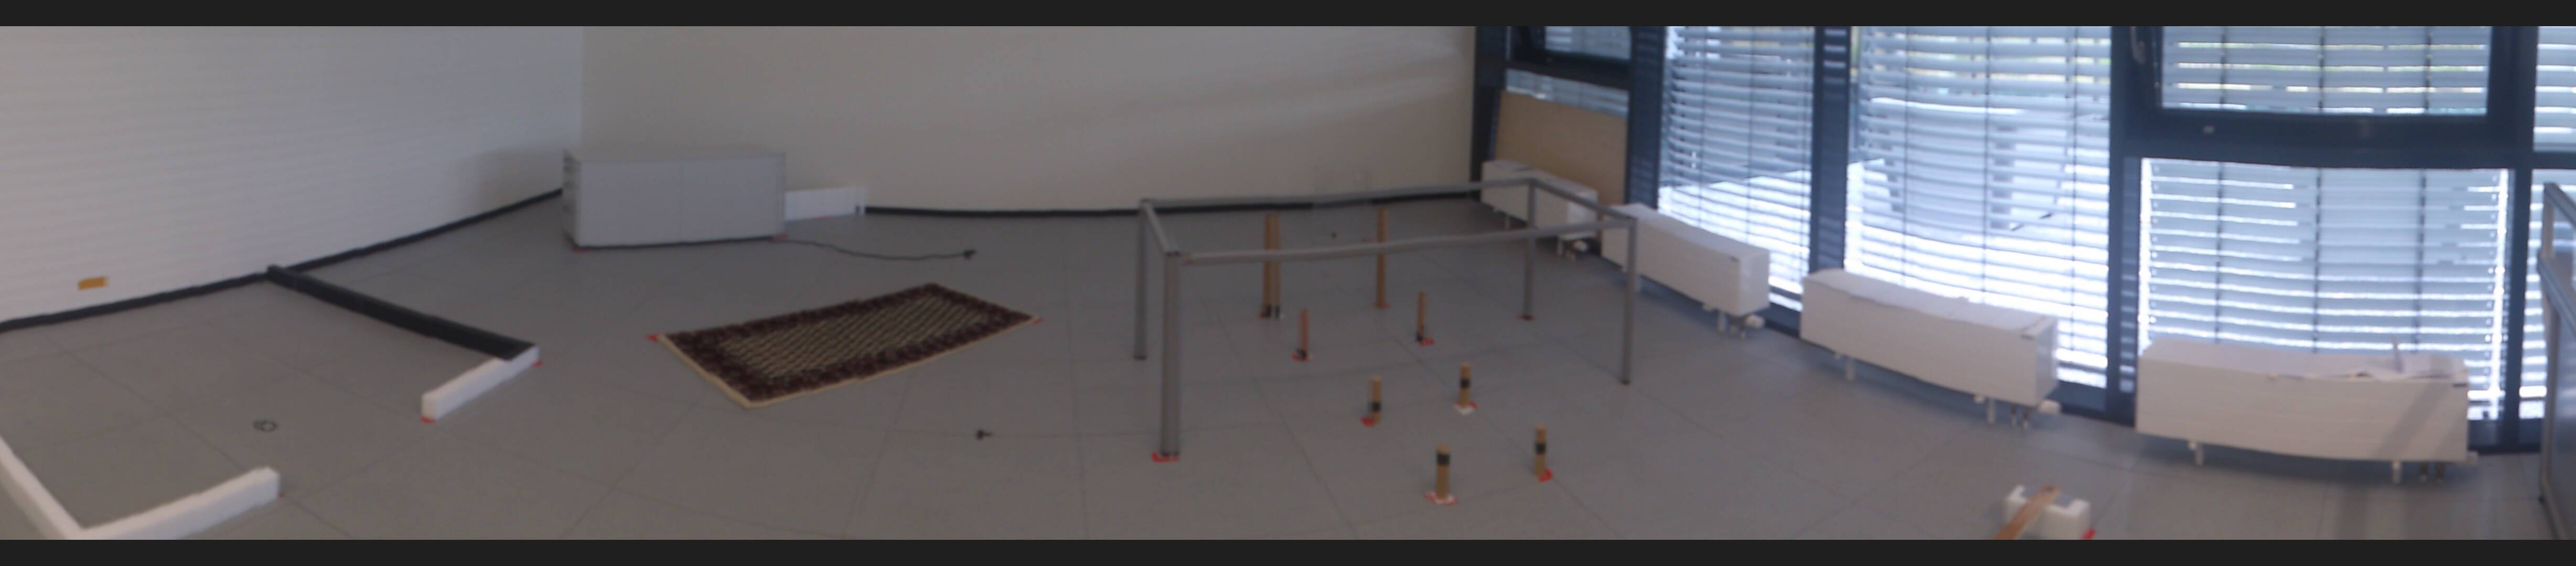
\includegraphics[width=\textwidth]{pictures/Setup_panorama.JPG}
	\caption{180$^\circ$ panoramic picture of the setup}
	\label{fig:panorama}
\end{figure}

In Fig. \ref{fig:scenario} you can see the setup stitched from the cameras at the ceiling and an overlay with the digitized scenario. The following enumaration provides detailed information about the marked positions:

\begin{enumerate}
\item Starting position: The starting position should be equal for all robots. Therefore the charging station was always placed at the position in the middle-bottom of the picture. This guarantees that the robots should all have the possibility to drive straight through the room after leaving the charging station at the beginning of the experiment. Left and right to the starting position the other robots wait in their charging station.

\item Small room: The small room offers at least three challenges. One challenge is the finding of the entrance of the room to simply test if the room is not left out while cleaning the rest of the area. Another challenge was the fact that the room might not allow to see the charging station from the inside what might perhaps produce unpredictable behavior in that case. The last challenge of the rooms was that some walls were white and some were black which could also lead to different treatments depending on the sensors which the robots use. 

\item Clearance height test: This obstacle should be a test if the robots recognize obstacle which they might not fit under. In fact in our case the obstacle was high enough that all robots were able to drive underneath without touching the obstacle. It would have been better if the obstacle would haven been adjusted individually to each robots height.

\item Small chair: We placed to chairs underneath our table to test the navigation in areas were the robots have lots of obstacles around them, which they should not touch or move around. The distances between the front and the back chair legs of the small chair do not allow any of the robots to get between them. They can only reach the area between from one of the sides (left/right).

\item Big chair: The big chair should test the same reactions as the small chair. The only difference is, that the distance between the individual legs allows the robots to get between them from all sides and also clean that area. 

\item Table: The table completes a stereotypical situation which will be part of most living rooms in the real world.

\item Carpet: The carpet is a real challenge for all of the robots. On the one side the robots have to overcome a height difference and on the other hand the material of the ground changes which may result in different driving characteristics. 

\item Loose cable (with fixated ends): Although in most of the manuals the user is advised to make sure that no loose cables may harm the robot in its cleaning area, we decided to include this in our scenario because it will often be the case in the real world and we wanted to investigate the behavior with this kind of obstacles.

\item Trap: The trap only offers a small entrance and may be a problem for robots which only use bump-sensors for navigation because it may take a while for them to get out of this area again. Therefore we wanted to measure the time which the robot spends inside the trap.

\item Glass cylinder: The material of this obstacle may be challenge for some kind of sensors which the robots use. We wanted to examine whether some robots bump against the cylinder or perhaps even move it around.

\item Heaters: The heaters were given obstacles in the room but they also provided some clearance height test and especially the heating controls turned out to be a problem for some of the robots.
\end{enumerate}

\begin{figure}[H]
	\centering
	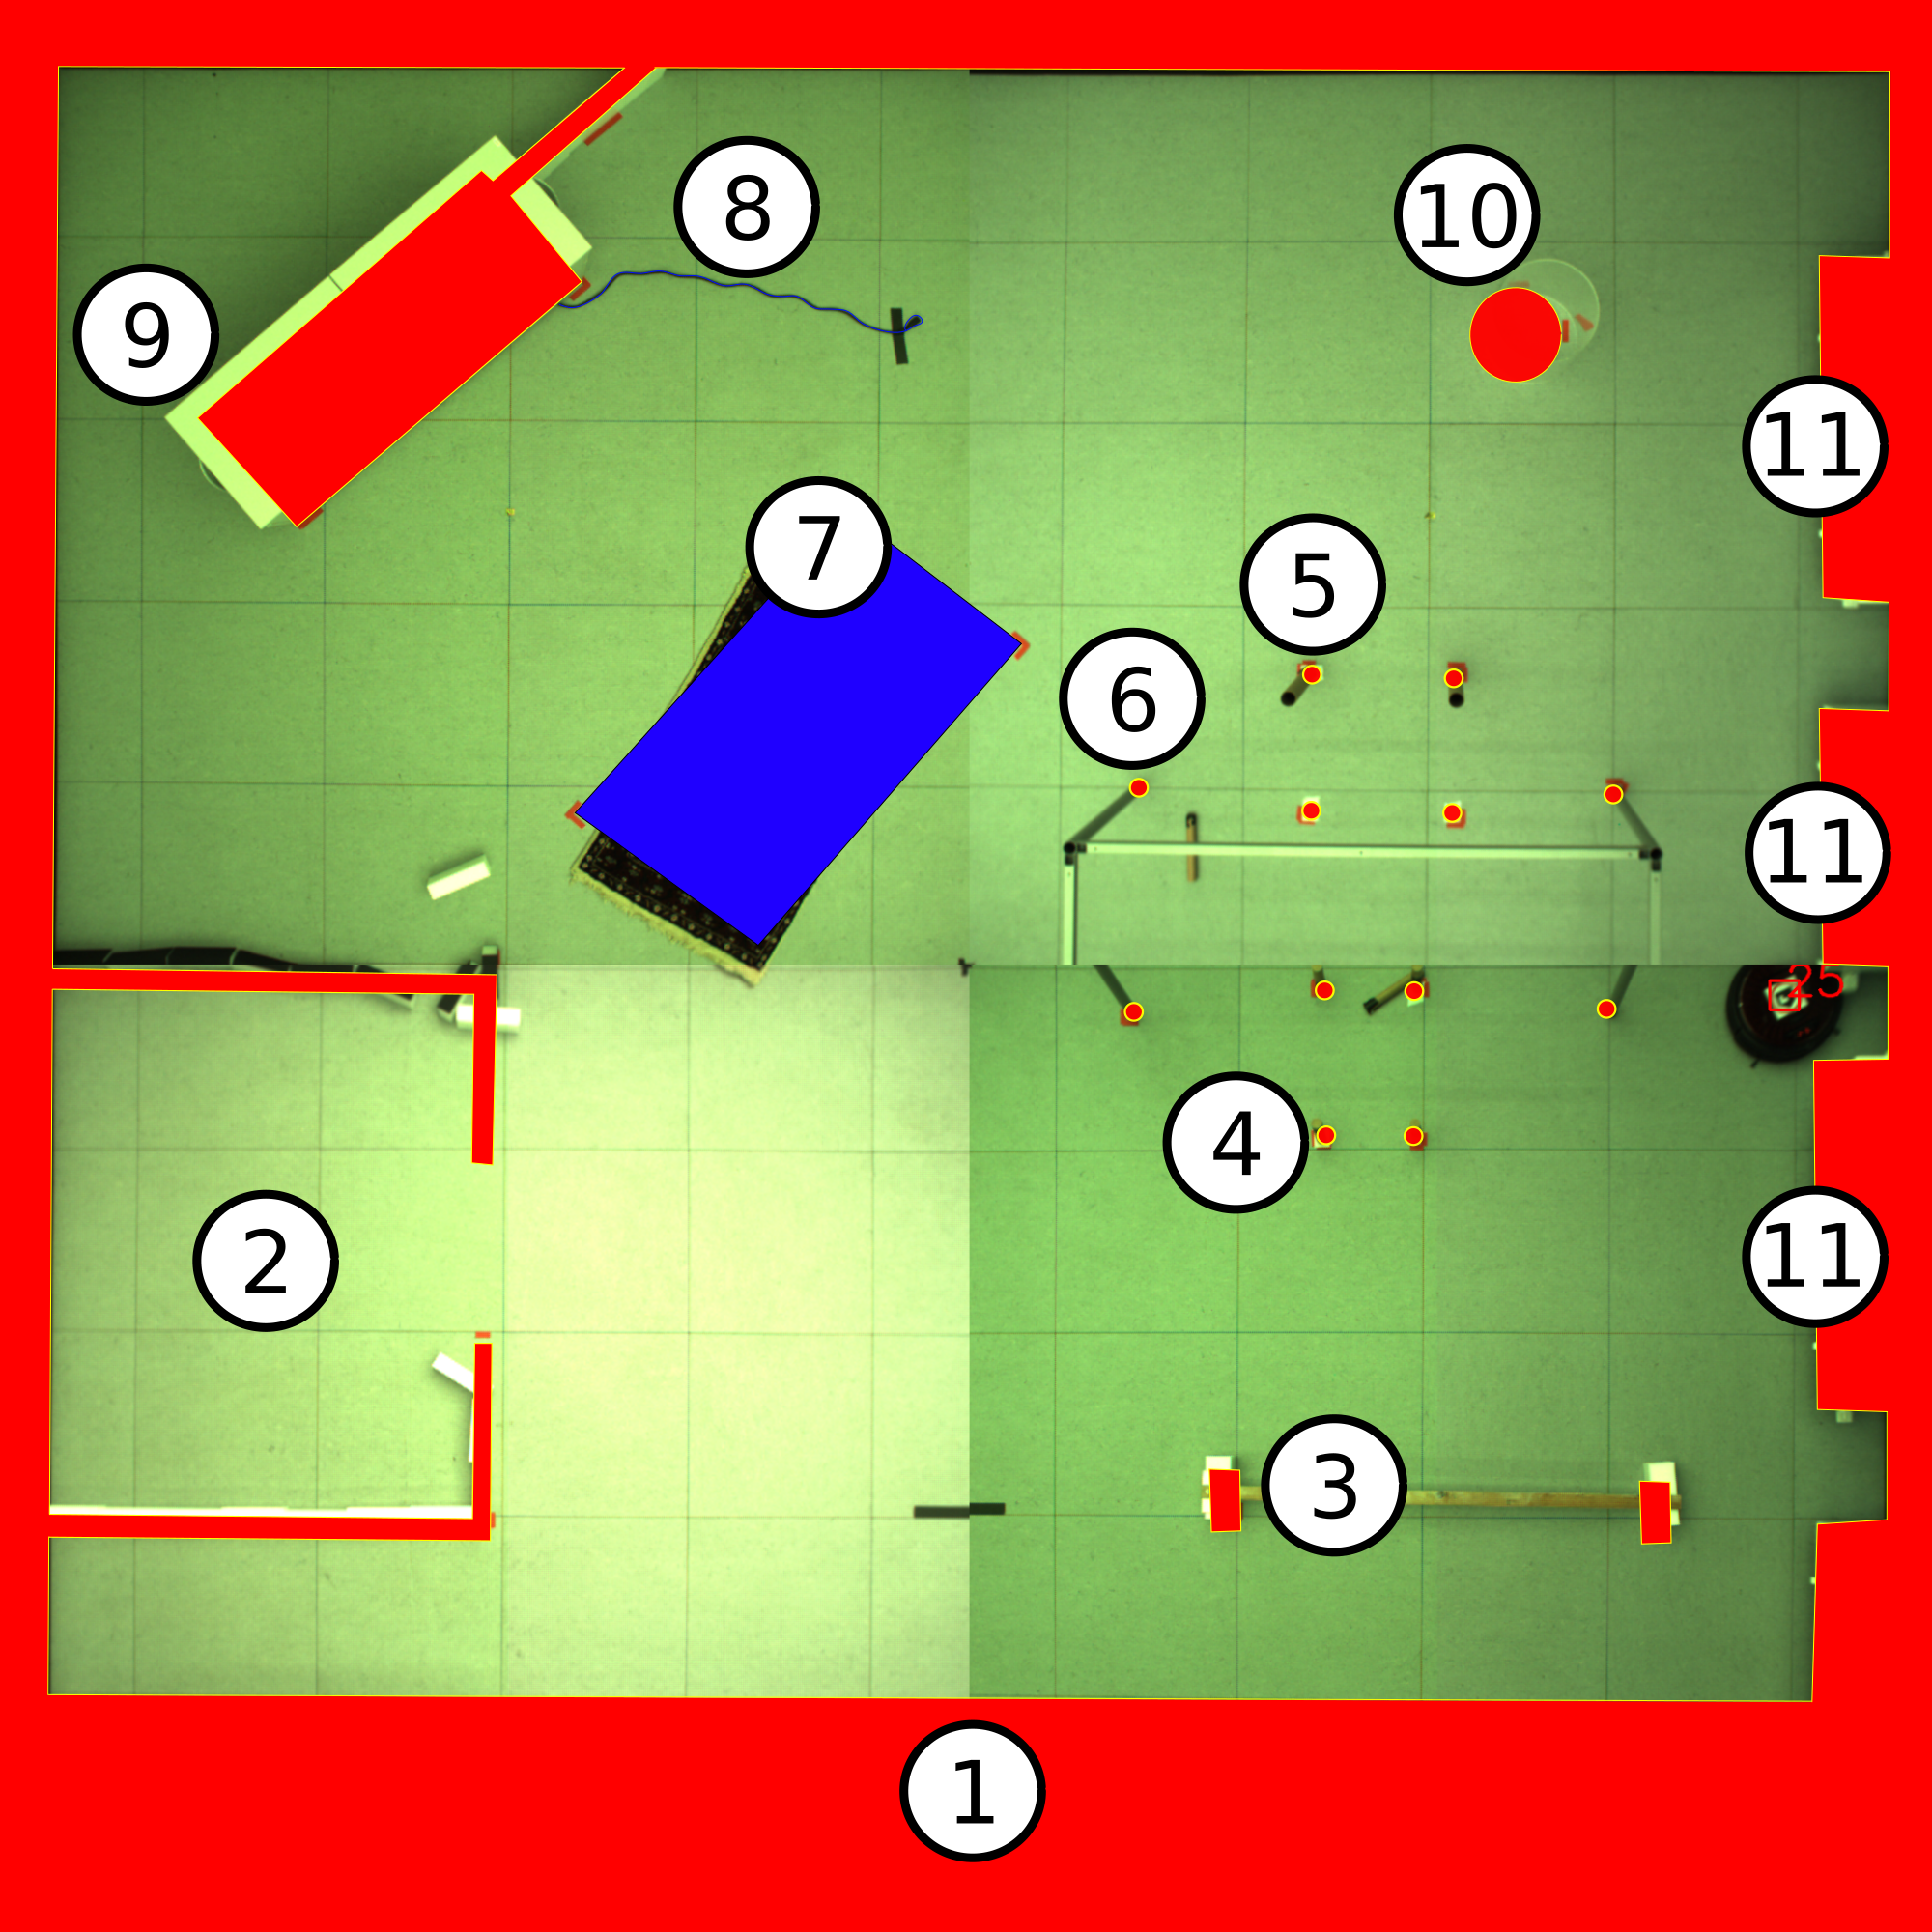
\includegraphics[width=0.5\textwidth]{pictures/senario_with_walls_picBack_labels.png}
	\caption{Sketch-overlay of the setup}
	\label{fig:scenario}
\end{figure}

\subsection{Tracking Tool} % Kosnoros
The tracking tool consists of four independent optical cameras, which are mounted to the ceiling and face towards the ground. Each camera provides a resolution of $1000 \times 1000$ pixel, bringing the total resolution to $2000 \times 2000$. A sample picture can be seen in Figure \ref{fig:setup}. Markers are glued to the objects that are to be tracked. Multiple objects can be tracked simultaneously. Each camera generates independent tracking data, which can be stitched with the other cameras' tracking data in the preprocessing step. Each entry in the tracking data contains the following elements:

\begin{itemize}
	\item Timestamp.
	\item Boolean value of either 0 or 1 depending on whether a certain marker was detected.
	\item The marker number. 
	\item X-coordinate.
	\item Y-coordinate.
	\item Turning angle.
\end{itemize}
X and Y-coordinates are given in pixel values that correspond to the marker position. 

\begin{figure} [H]
	\begin{center}
		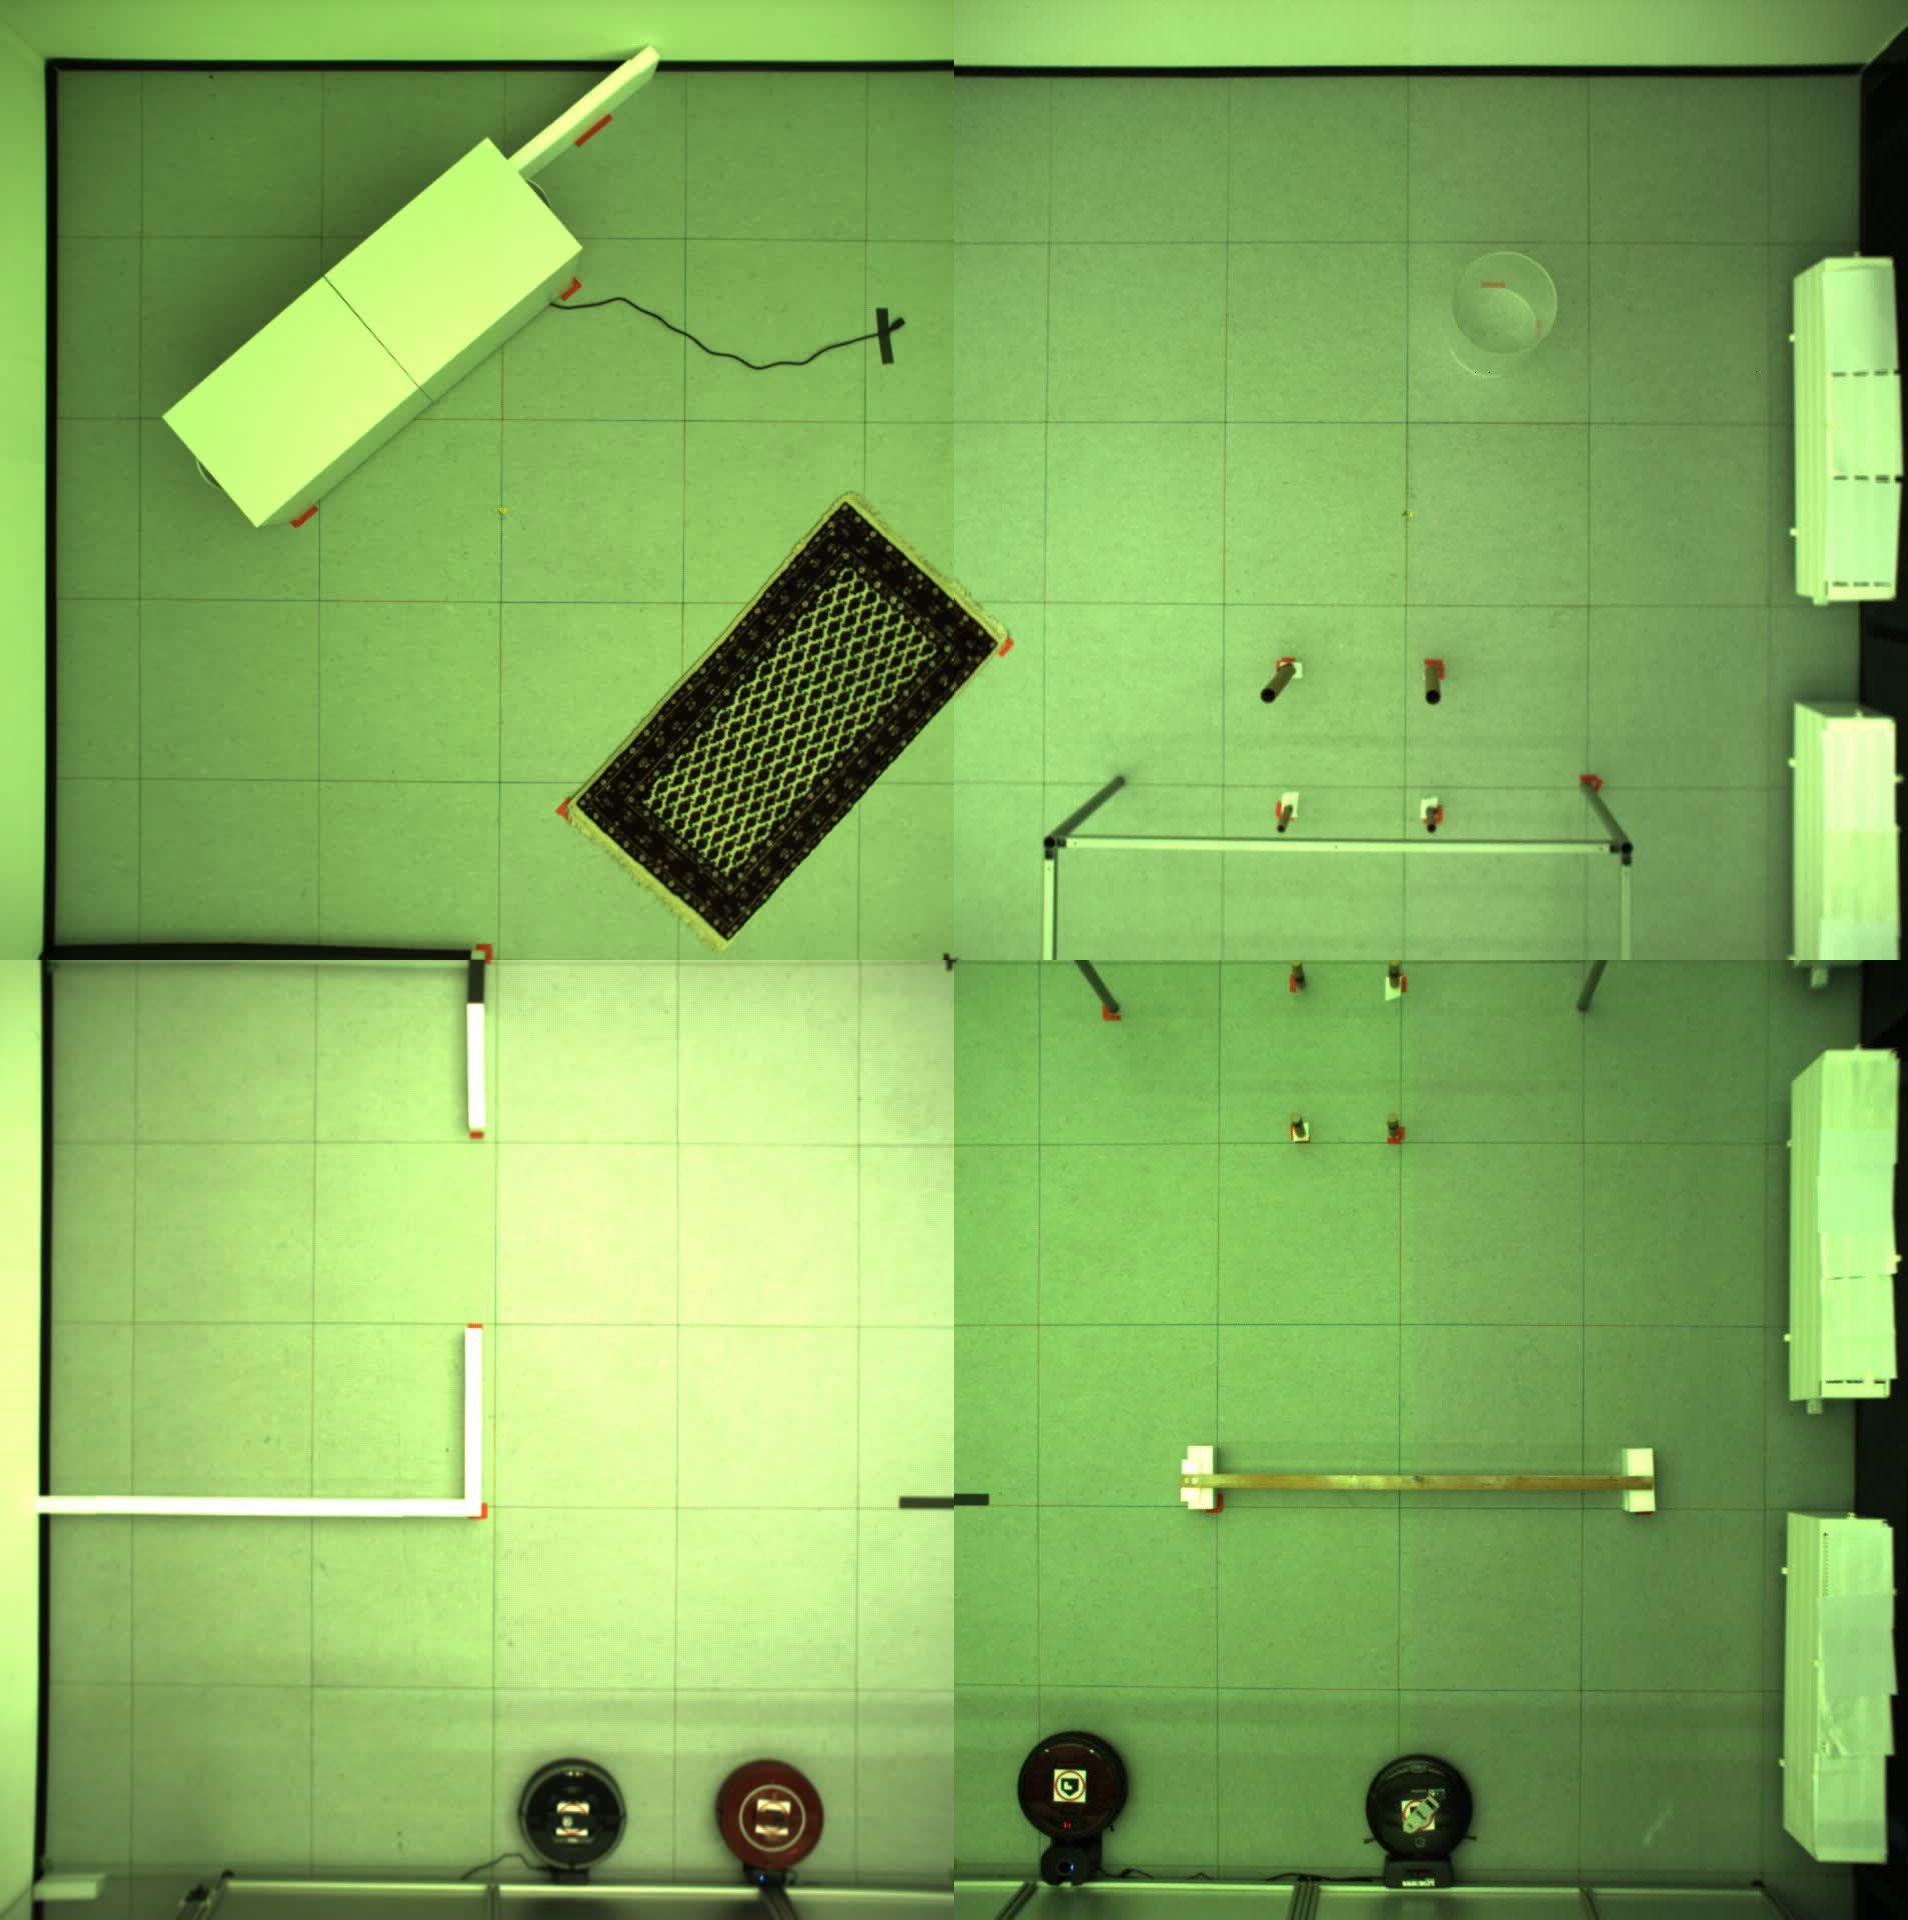
\includegraphics[width=0.5\textwidth]{pictures/setup.jpg}
		\caption{Exemplary camera picture.}
		\label{fig:setup}
	\end{center}
\end{figure}


\subsection{Execution} % TODO Andi
Before some tracking data can be collected with the tracking tool, there must be prepare the scenario and start the tool.

\subsubsection{Cameras and light}
The first step is to prepare the cameras, if they are off. That means to turn-on all of the cameras and wait for 2-3 minutes. In these time, the server of the teleworkbench is assigning a IP address for each camera.

The next step is to turn-on the teleworkbench lights above the test area to get a better tracking quality. This can be done via the DALI web-interface, where every light can be switch on/off by pressing the related button.

\subsubsection{Start GUI of the tracking tool}
By a double click on the short cut \textit{TWB\_GUI\_VIDEO\_AND\_TRACK\_RECORD} the teleworkbench GUI opens. To record a new video and track data, the button \textit{Access the Cameras} should be pressed. Hereupon will be pop up a window as reminder that you have to wait for few seconds, which can be click away by \textit{OK}. Now, the tracking tool is ready to track data and the next \textit{OK} button starts the tracking process. Before the start button is pressed, the robot should be placed in the center of the robots at the red marker, like in figure \ref{fig:place}. In addition to allow tracking, a marker must be placed (and better taped) on the robot. An important point is that there is no one inside the TWB area in the beginning when the tracking tool starts. If everything is fine, the tracking can be started via the \textit{OK} button and at once,the robot should be started via remote control too.

\begin{figure} [H]
	\begin{center}
		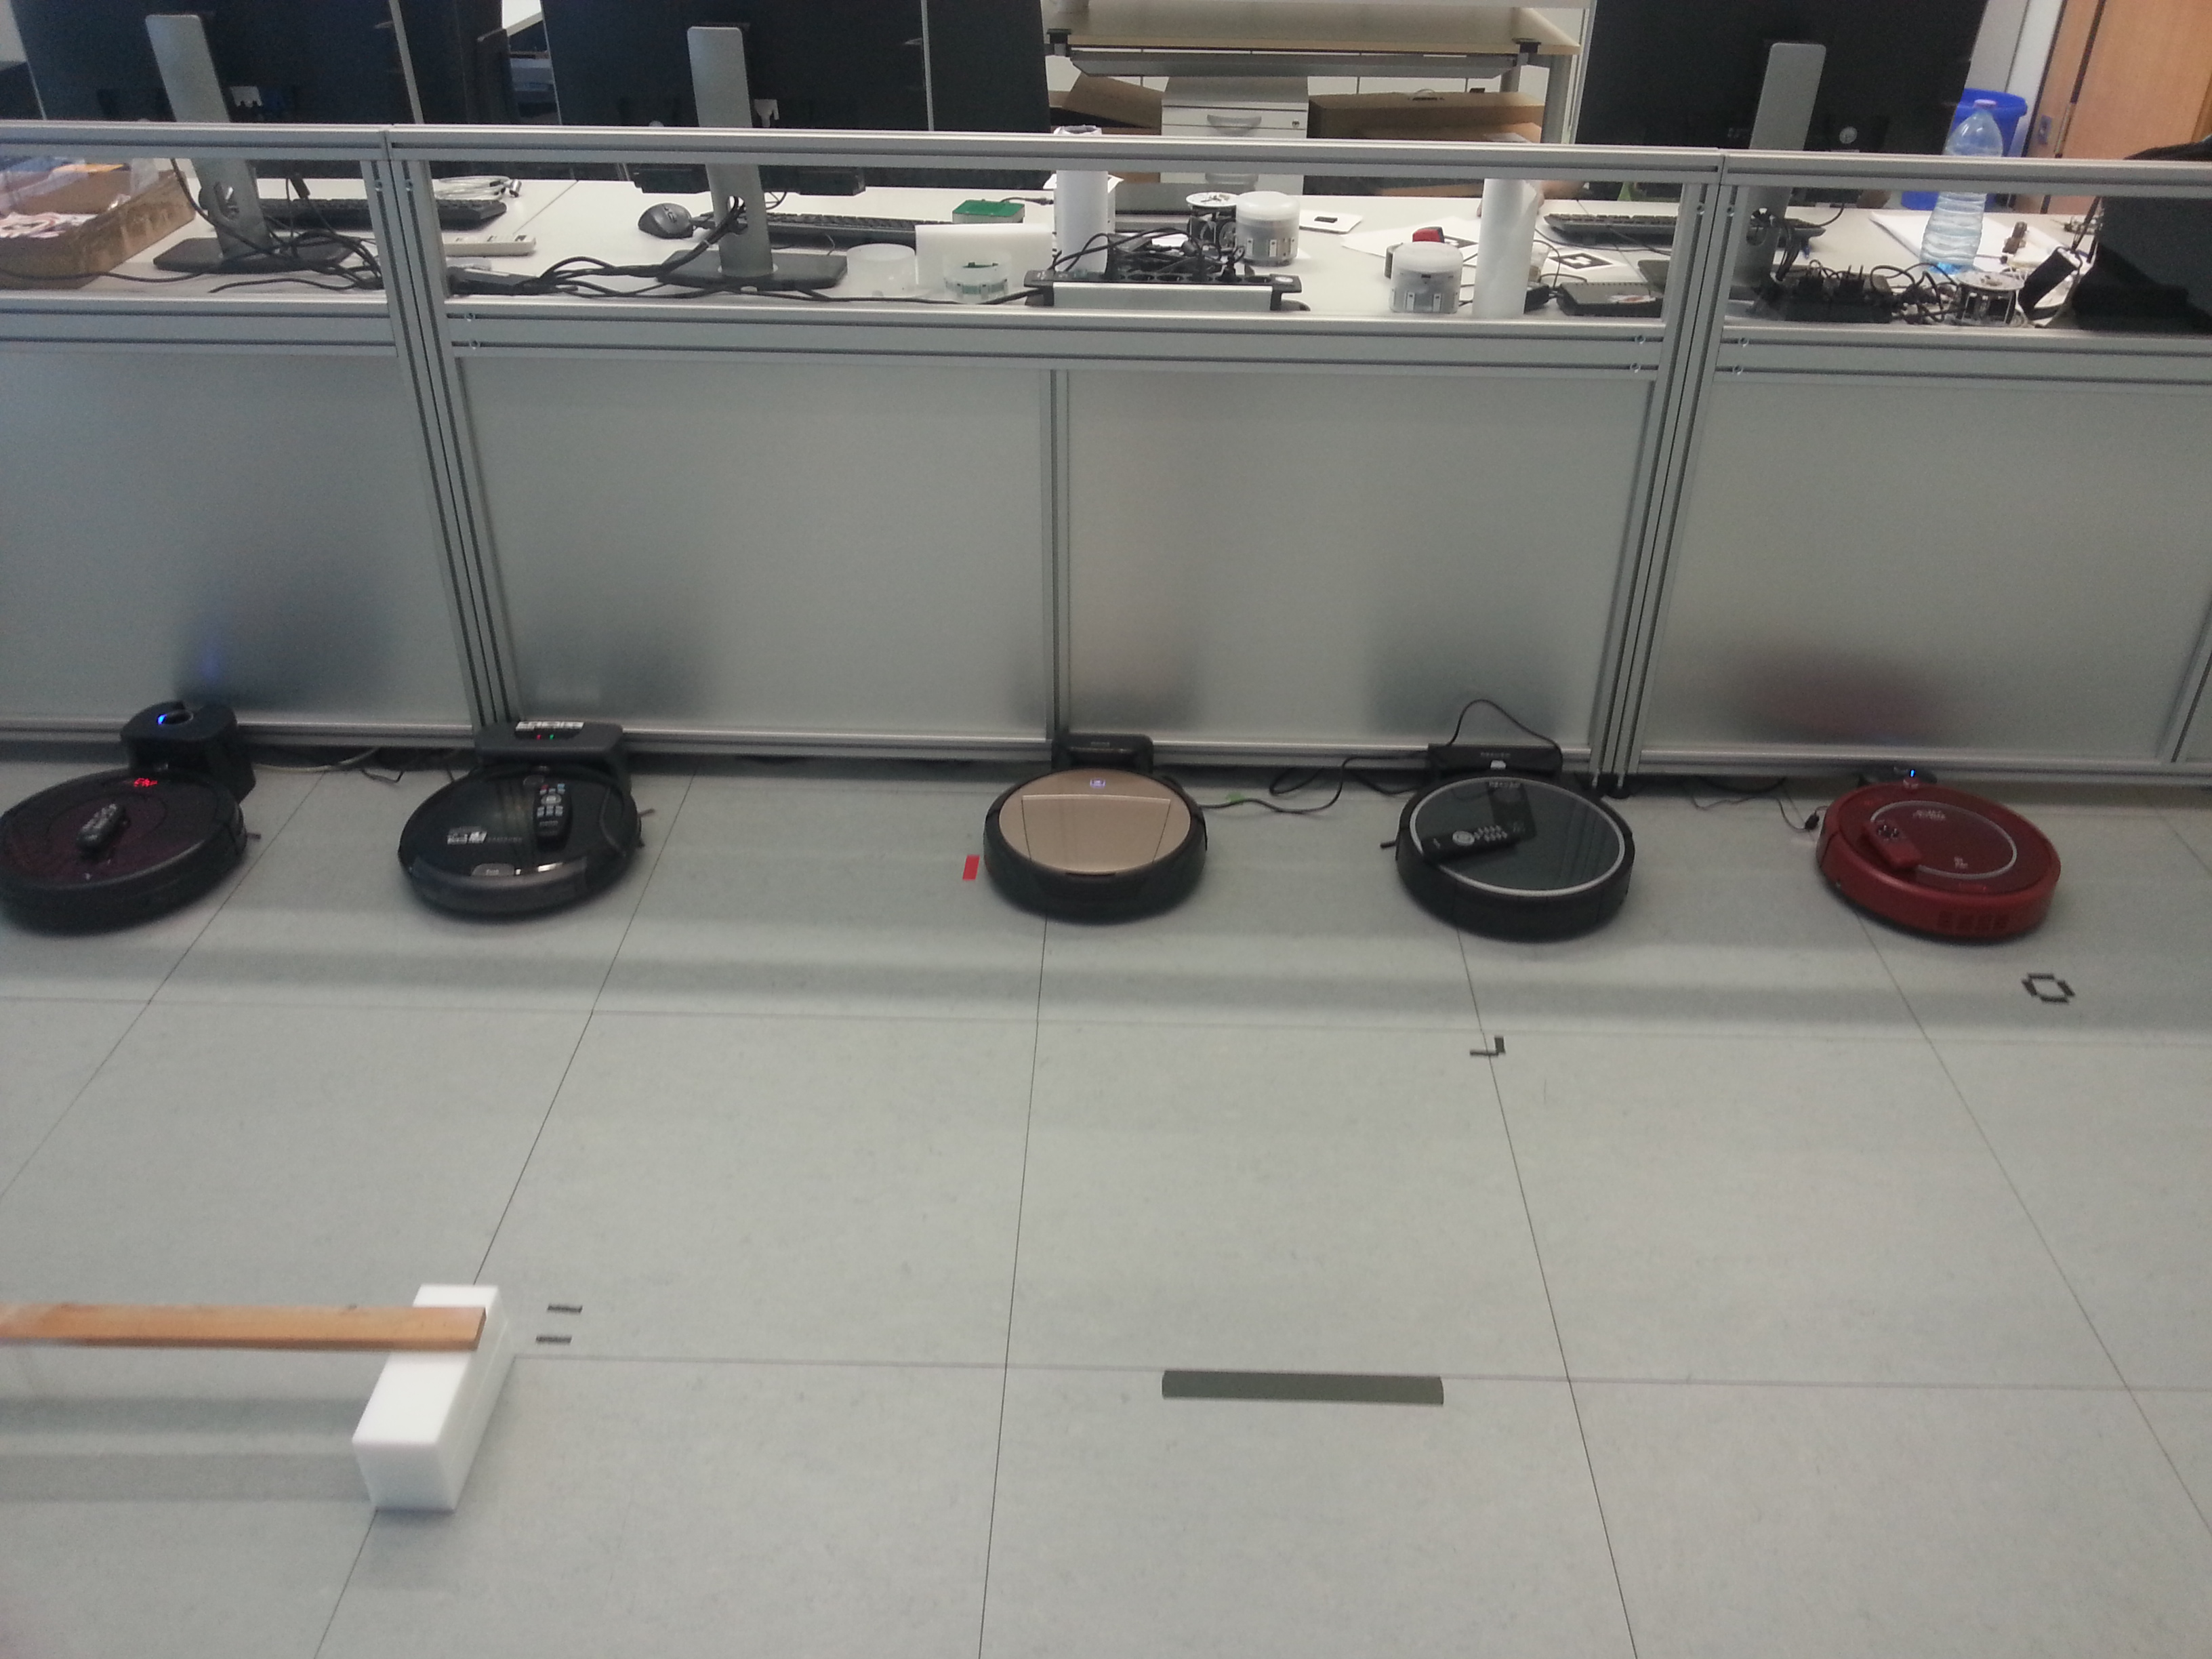
\includegraphics[width=0.5\textwidth]{pictures/place.jpg}
		\caption{Start position of the robot with the charging station.}
		\label{fig:place}
	\end{center}
\end{figure}

If the cleaning process of the robot is done, the tracking process should be stopped via pressing the \textit{ESC} key. Now, you can get the tracking data, which are in the folder \textit{D:\textbackslash ASE\_ProjectVideo\_TWB\textbackslash RecordingDateandTime}.

\section{Evalution Algorithms}
\subsection{Group 1}
\subsubsection{Preprocessing of tracking data} % TODO Hendrik
The tracking data came from an external application and consisted of four simple textfiles with the following format for each line:
\[(Time:HHMMSS.MS) (\#Tracked markers) [(Tracker ID) (Angle) (X_{Position}) (Y_{Position})] \]
Which looks like this for a concrete case:
\begin{center}
\texttt{222202.405827\ 1\ 32\ 270\ 87\ 897}
\end{center}
Our first task was to combine the data from all four text files and create one representation which contains the tracking data relative to the complete area. 

We decided to use a \texttt{QMap} for that because it is an ordered combination of a key and a value. In our case the key is the complete timestamp and the values are vectors which contain the angle and the x and y position. This way it was easy to combine the tracking data in one representation because we could assume that nearly no timestamps are equal and if they are, their tracking data should be very similar so that storing only one of them should be sufficient.

Our approach was to successively iterate over all lines of the four files and then check whether the line holds meaningful data. If it does, the values from the line are extracted with simple string operations and an offset is added to the x or y position or to both, depending on the file where they were coming from. At the end of the extraction we had all we need: A timestamp for the key and the relative position and orientation (not needed any further) for our vector.

Later we added a scaling factor to the x and y position because the tracking data does not provide values between the full range from 0-1000. This results from the fact that the pictures for the tracking data are stitched together and because of the overlap the tracking data can not reach its maximum values. The scaling factor is multiplied to the x and y positions before adding the offset.

All of this is done in the method \textit{\texttt{extractData(...)}}. It is called four times (for the four files) from the method \textit{\texttt{preprocessTrackingData()}} inside the \textit{\texttt{VacCleanAnalyzer}} class.

\subsubsection{Distance} % TODO Andi
One task is to compute the distance of the robot during a cleaning process, which based on the tracking data.

First of all the \textit{\texttt{VacCleanAnalyzer}} class generates an instance of the \textit{\texttt{Coverage}} class. The relevant values are the X- and Y-coordinates. The main idea is that the distance between two successive tracking points is computed and add them together. The distance between the two points is realized via Pythagorean theorem in the \textit{\texttt{Distance::updateDistance(...)}} method. That means in the first cycle the distance is the first point, because their are no two points. But now every cycle the Pythagorean theorem sets a new distance and then the method add the new distance value with the old distance value together.


At every time, the current distance can be get via the call of \textit{\texttt{Distance::getCurrentDistance()}} method and \textit{\texttt{Distance::getDistanceInM()}} method in pixels and in meters.

\subsubsection{Duration} % TODO Timo
To analyse how much time passed until a certain point of the tracking data, another task was to calculate the elapsed time between the first and the current data point.

The \textit{\texttt{Duration}} class provides this functionality to the \textit{\texttt{VacCleanAnalyzer}} class. 
Relevant for this class are the two timestamps which are split into hours, minutes and seconds. The first one is the referencing timestamp to which the difference is calculated. The second one is the current timestamp.
Within the iteration over the tracking data, the timestamp of the current data, which is stored as the key of the \texttt{QMap}, is passed to the \textit{\texttt{Duration::updateDuration(...)}} function. If called for the first time, the function stores the given timestamp as the referencing one. With every following call of the function, the current timestamp is overwritten with the one.

The class also provides two functions, which return the current duration. The function \\ \textit{\texttt{Duration::getCurrentDuration()}} provides the passed time in seconds and the \\ \textit{\texttt{Duration::getFormattedDuration()}} function formats the duration into the "HH:MM:SS" format. The main functionality of this methods are similar. They both calculate the duration by calculating the difference of the current timestamp to the first one. 

At any stage of the iteration it is possible to call this functions and get to know how much time is passed until this data point.

\subsubsection{Coverage} % TODO Julian D.

Another task was to precisely calculate the percentage the robot covered until a certain amount of tracking points.

In order to achieve this, the \textit{\texttt{VacCleanAnalyzer}} class first generates an instance of the \textit{\texttt{Coverage}} class.
Height and width of the tracking image, as well as the diameter of the robot in centimeters are passed via parameters.
While iterating over the tracking data, the tracking points are then successively passed to the \textit{\texttt{Coverage::updateCoverage(...)}} method.
In this method a green line is drawn from coordinate to coordinate onto an empty image with the dimensions of the tracking image.
The thickness of this line corresponds to the diameter of the robot.

At any arbitrary point it is possible to call the \textit{\texttt{Coverage::getCurrentCoveragePercent()}} method, in which the current precentage of the coverage will be calculated depending on the amount of green pixels in the image.
Additionally it is possible to provide a scenario model to the program.
This scenario image has to look like the red overlay which is already shown in Figure \ref{fig:setup}.
Every pixel pointed in red will then not be consulted for the coverage calculation, leading to the fact that the resulting percentage only depends on the area, that the robot theoretically could have reached.

Furthermore it is possible to export the coverage image at any time.
In order to do so the \textit{\texttt{Coverage::exportScenarioAndCoverageImage(...)}} method has to be called.
A combination of the scenario and of the coverage image will then be created and saved under the given filename.
Examples of these images can be seen in Figure \ref{fig:coverage}.

\begin{figure}[H]
	\centering
	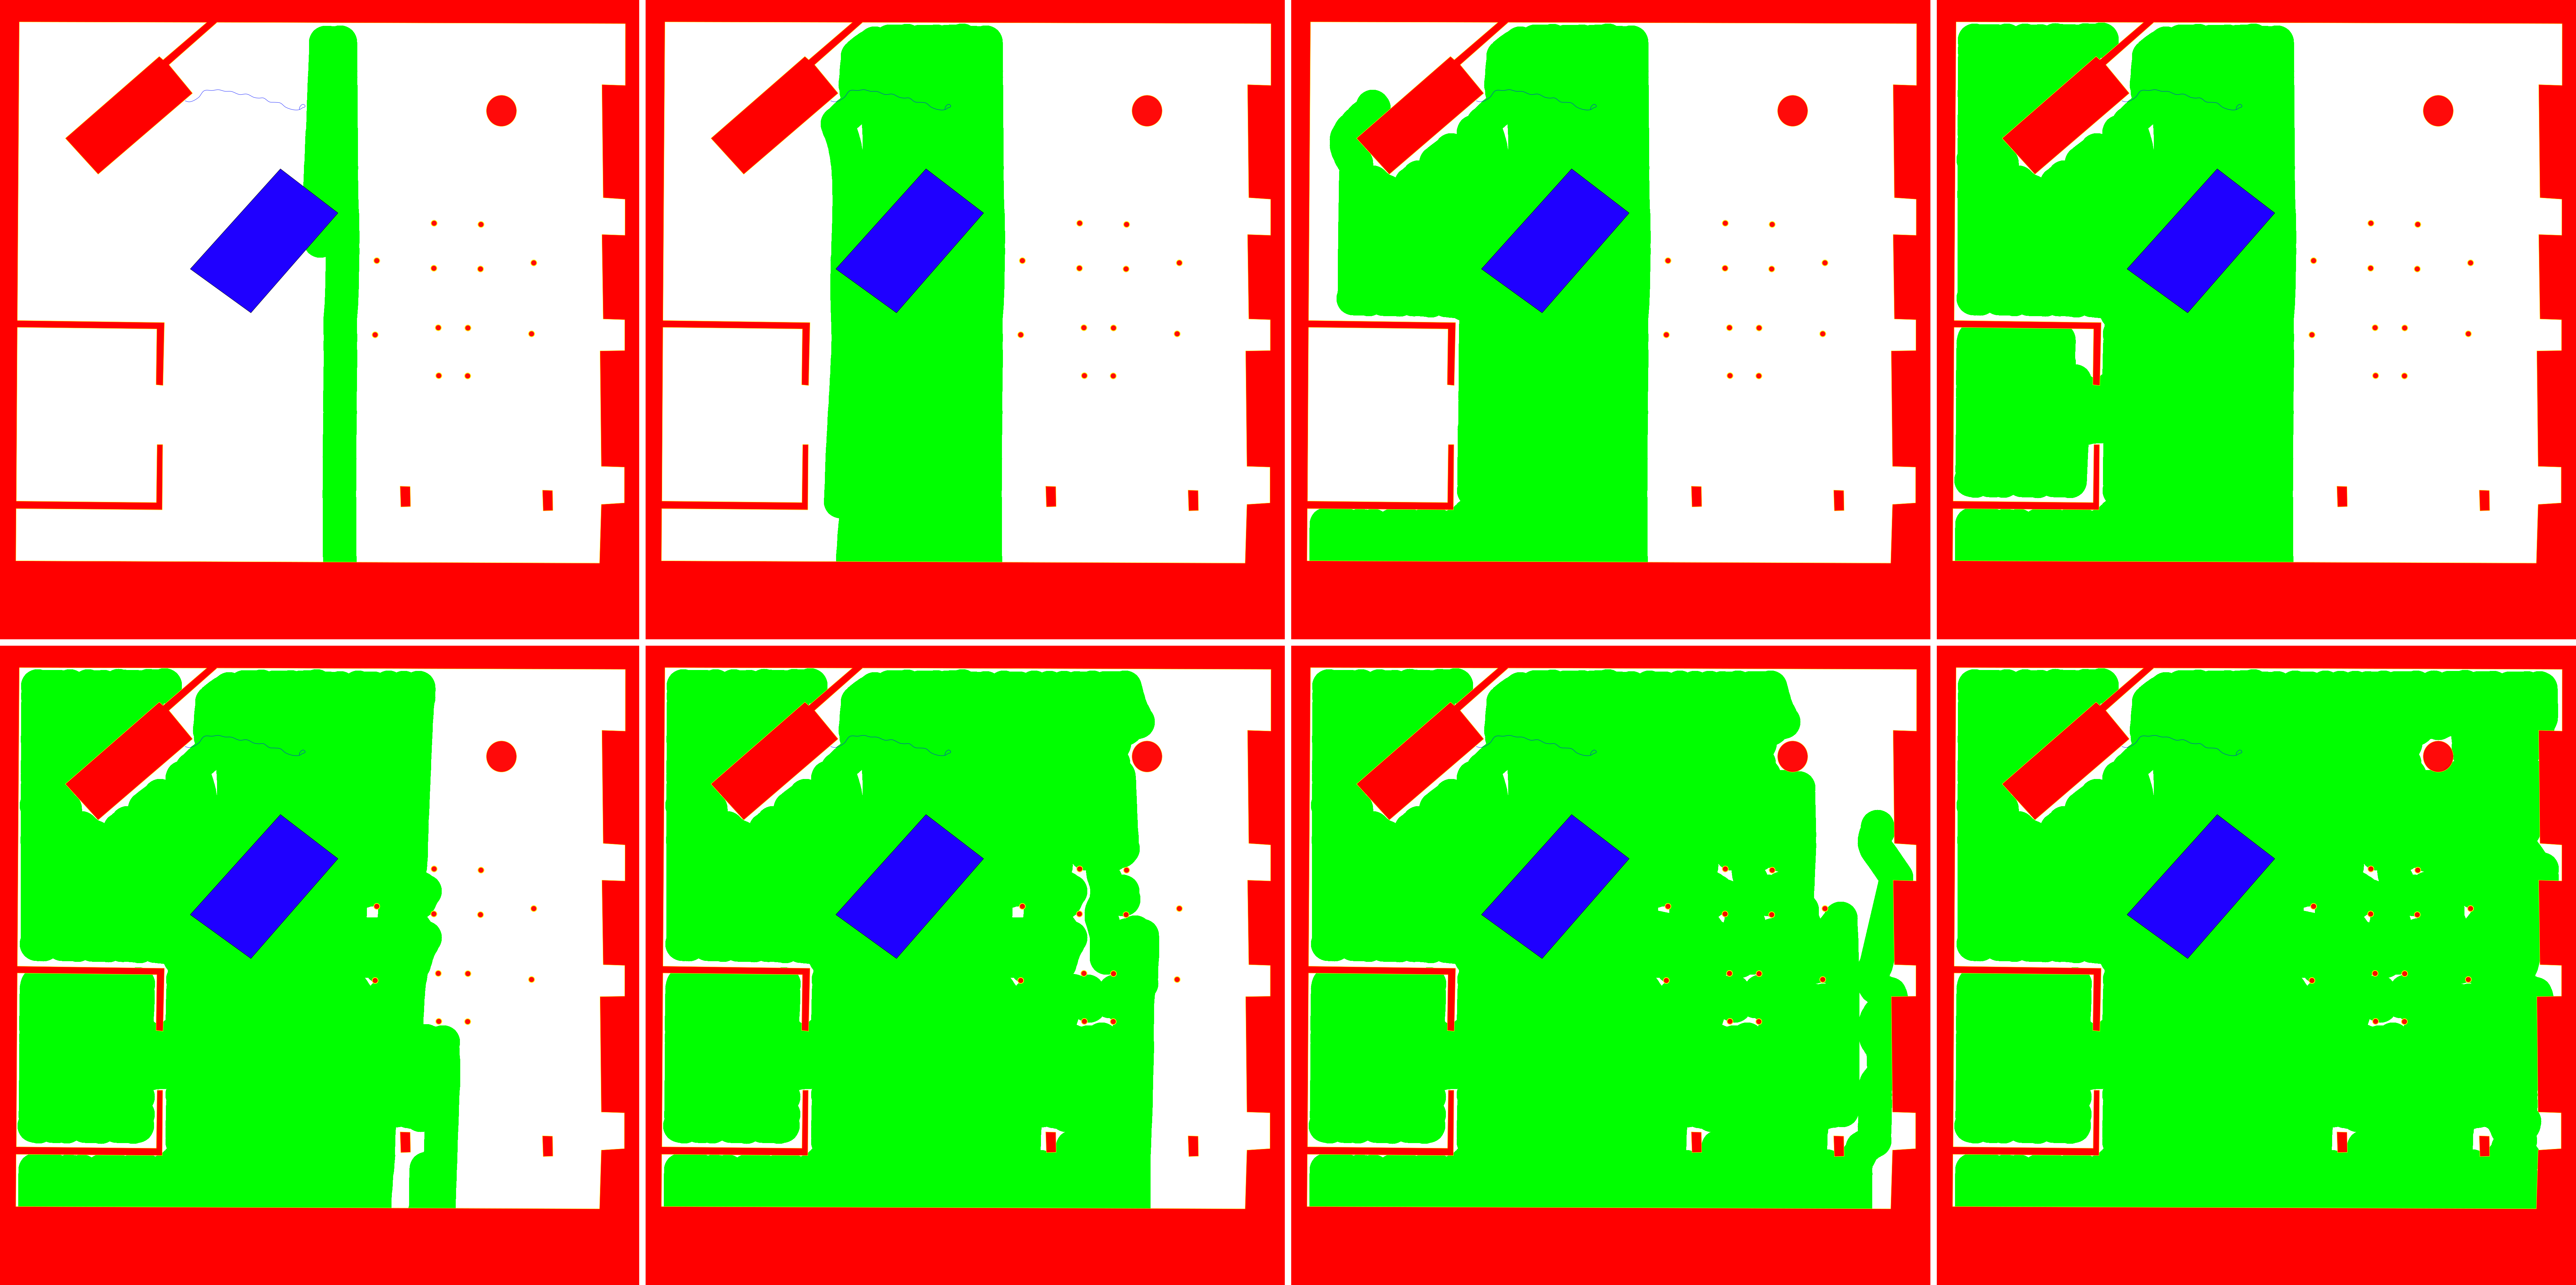
\includegraphics[width=\textwidth]{pictures/coverage_process.png}
	\caption{Coverage example of the Miele Scout RX1 (interval of 5 minutes)}
	\label{fig:coverage}
\end{figure}

\subsubsection{Heatmap} % TODO Leroy

\subsection{Group 2} % TODO Julian E. & Martin
\subsubsection{Preprocessing of tracking data}
\subsubsection{Heatmap}
\subsubsection{Histogram}

%\end{multicols}

\end{document}
